\section{Tahap Simulasi dan Optimasi}
\label{sec:tahap-simulasi-optimasi}

\begin{figure}[!ht]
    \centering
    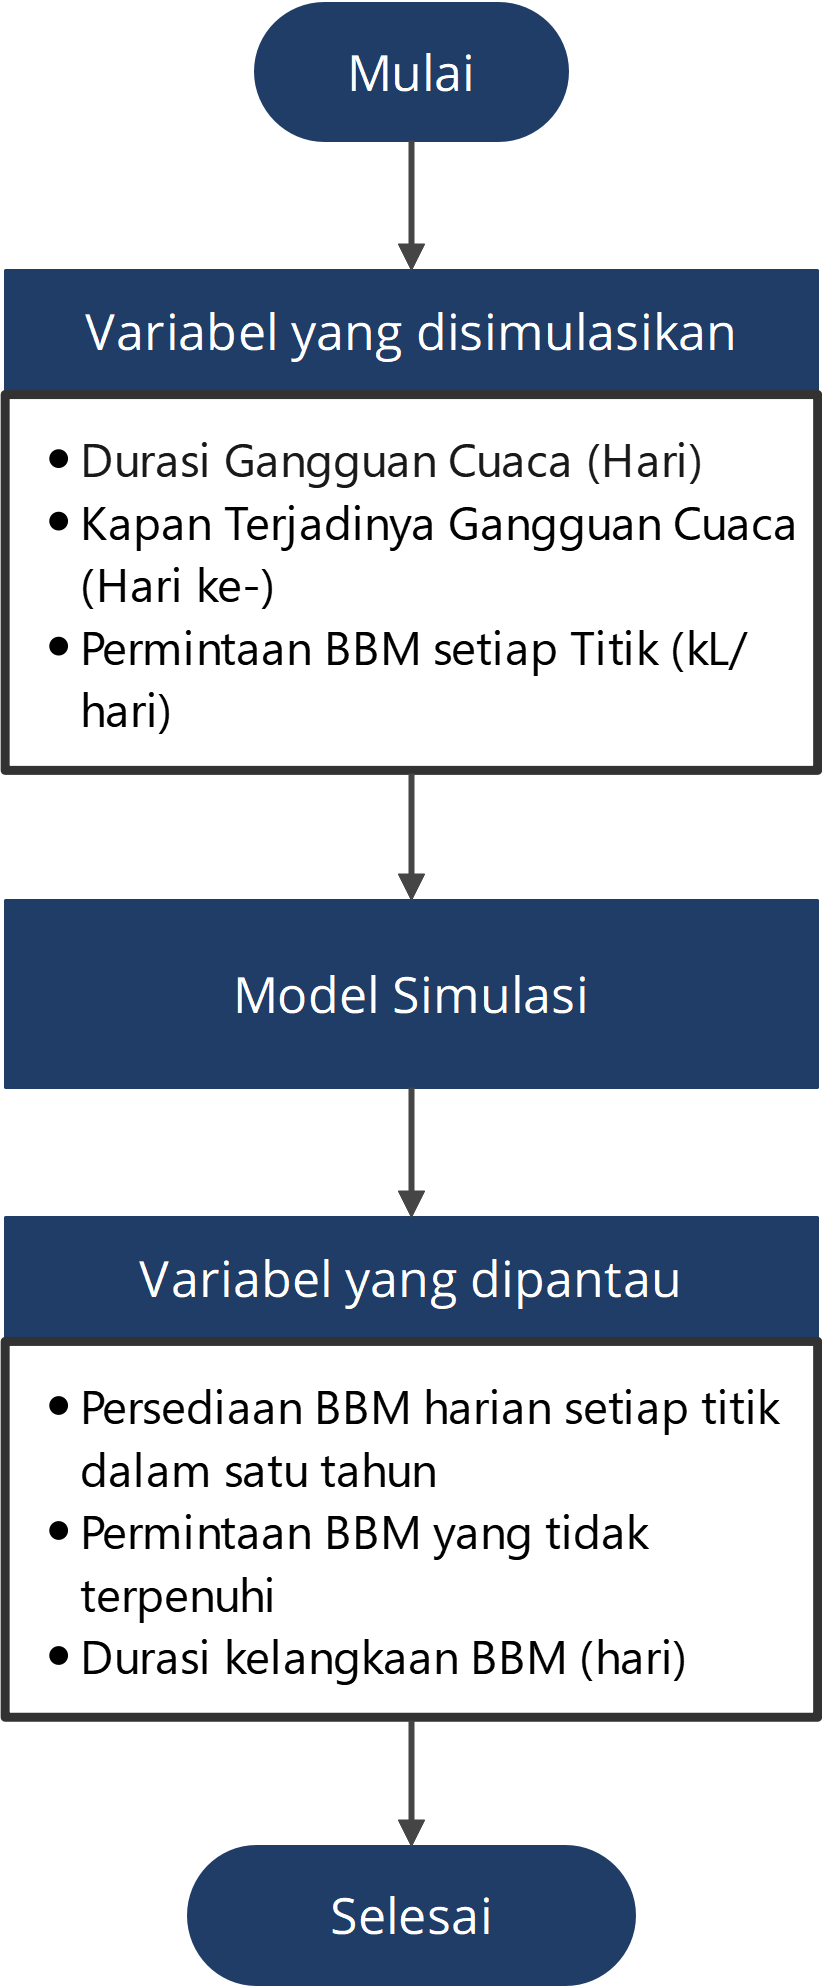
\includegraphics[width=0.25\textwidth]{gambar/FC_Simul.png}
    \caption{Diagram Alir Simulasi}
    \label{fig:flowchart-simulasi}
\end{figure}

Simulasi dilakukan untuk menguji kondisi sistem pemasokan yang sudah ada. Metode ini dipilih untuk mencoba memotret kondisi lapangan yang ada dan melakukan analisis terhadapnya. Selain untuk mengevaluasi sistem yang sudah ada pada proses perancangan kapal yang baru juga dilakukan simulasi untuk parameter desain dilengkapi dengan model optimasi.

\subsection{Tahap Simulasi}
\label{subsec:tahap-simulasi}

    Informasi yang sudah didapat dari studi literatur dan studi lapangan kemudian dijadikan bahan untuk untuk membuat model. Penulis sendiri membagi pengerjaan menjadi dua model; model perancangan kapal dan model skenario penyaluran BBM.

    Model perancangan kapal berisi berbagai macam langkah perhitungan yang digunakan untuk merancang kapal dari \emph{owner requirement} hingga menjadi desain awal sebuah kapal. Pembuatan model ini bertujuan sebagai batasan ruang lingkup saat nanti akan dilakukan proses optimasi. Batasan yang diterapkan dalam model ini adalah kaidah-kaidah dasar perancangan kapal.

    Model kedua adalah model perancangan skenario penyaluran BBM. Model ini mencakup rencana operasional dan pemodelan finansial kapal yang dirancang. Interaksi atau hubungan antara sisi teknis, operasional dan finansial ini yang akan menjadi proses optimasi perancangan kapal. Model kedua ini juga membahas masalah penentuan tambahan kapasitas penyimpanan BBM jika diperlukan oleh suatu titik.

    Sisi simulasi monte carlo akan dilakukan dengan cara menentukan masukan yang akan divariasikan kedalam model. \emph{Input} yang akan divariasikan dalam penelitian ini adalah data konsumsi BBM perhari untuk setiap titik dan durasi gangguan cuaca tiap tahunnya. Harapannya dengan variasi dari masukan tersebut dapat memotret kondisi sebenarnya yang terjadi di lapangan.

    Variasi \emph{input} dilakukan dengan cara memetakan distribusi dari \emph{input} yang ingin divariasikan. Disini, penulis menggunakan data historis yang didapat penulis untuk mengidentifikasi distribusi dari \emph{input} yang diinginkan. Metode peramalan yang digunakan penulis adalah \emph{Three Point Estimate} dengan alasan utama, metode dan distribusi peluang tersebut mudah dipahami dan diterapkan.

    \emph{Input} yang sudah divariasikan tersebut kemudian diintegrasikan kedalam model kedua, yakni model perencanaan operasional kapal. Proses berikutnya adalah menetapapkan vaiabel apa yang akan dijadikan sebagai luaran dari proses simulasi. Sesuai dengan tujuan penelitian luaran yang akan dipantau adalah ekspektasi biaya tahunan, kemungkinan permintaan BBM yang tidak terpenuhi dan kemungkinan terjadi kelangkaan BBM di suatu titik.

    Model kemudian diuji coba dengan iterasi yang ditentukan untuk mendapatkan data kumulatif frekuensi dari luaran yang dipantau. Proses iterasi dilakukan dengan bantuan perangkat lunak \emph{Microsoft Excel} dan \emph{Palisade @RISK Platform}. Jika model sudah berjalan dengan lancar, pengerjaan dapat dilanjut pada tahap berikutnya.

\subsection{Tahap Optimasi}
\label{subsec:tahap-optimasi}

    Metode optimasi digunakan untuk mencari nilai paling optimal dari kompromi berbagai macam batasan yang muncul saat proses perancangan kapal secara teknis maupun ekonomis. Fungsi tujuan optimasi yang dilakukan dapat dilihat pada formulasi matematis berikut.

    \begin{equation}
        \min\sum_{p\in P}\sum_{i\in N}A_{i,p}+\sum_{\mathrm{x}\in X}\sum_{i\in N}Y_{i.t}+OC+FC+SOC+PC
        \label{model-matematis-optimasi}
    \end{equation}

     dengan memenuhi batasan-batasan berikut:

\begin{align}
    5.1 \leq \frac{L}{B} &\leq 7.1 \label{crasio1} \\
    2.4 \leq \frac{B}{T} &\leq 3.2 \label{crasio2} \\
    10 \leq \frac{L}{T} &\leq 30 \label{crasio3} \\
    0.669 \leq \frac{T}{D} &\leq 0.799 \label{crasio4} \\
    1.9 \leq \frac{B}{D} &\leq 2.1 \label{crasio5} \\
    D &\geq \frac{L}{16} \label{crasio6} \\
\end{align}
\begin{align}
    e_{0,30^\circ} &\geq 0.06 \label{cstabil1} \\
    e_{0,40^\circ} &\geq 0.09 \label{cstabil2} \\
    e_{30,40^\circ} &\geq 0.03 \label{cstabil3} \\
    h_{30^\circ} &\geq 0.20 \label{cstabil4} \\
    \phi_{max} &\geq 25 \label{cstabil5} \\
    GM_0 &\geq 0.15 \label{cstabil6} \\
    D - T &> \text{Freeboard}_{\text{min}} \label{cfreeboard} \\
    0.5\% W_{\text{total}} &\leq \Delta_{\text{Displ}} \leq 5\% W_{\text{total}} \label{cberatkapal} \\
    0.5\% V_{\text{payload}} &\leq \Delta_{\text{Volume}} \leq 5\% V_{\text{payload}} \label{cvolumekapal} \\
    -1.5\% L_{\text{PP}} &\leq \text{Trim} \leq 1.5\% L_{\text{PP}} \label{ctrim} \\
    \text{Seatime} + \text{Porttime} &> \text{Leadtime} \label{cwaktu1} \\
    \text{Required Time} &> \text{Comission Days} \label{cwaktu2}
\end{align}

    Fungsi tujuan dibuat untuk mencari biaya total paling minimum. $P$ melambangkan himpunan pelabuhan yang disinggahi. $N$ melambangkan titik pemasokan. $A$ melambangkan biaya pelabuhan yang muncul akibat kapal beroperasi. $X$ adalah himpunan ukuran tangki. $Y$ adalah biaya pembangunan tangki yang sudah dikonversi menjadi bentuk biaya tahunan. $OC$ melambangkan biaya operasional kapal atau biaya tetap kapal yang dikeluarkan tahunan. $FC$ adalah biaya BBM yang keluar akibat operasional kapal dalam setahun. $SOC$ dan $PC$ masing-masing adalah biaya penalti yang muncul jika terjadi kelangkaan BBM dan muatan yang tidak mampu diangkut oleh kapal.

    Variabel peubah yang digunakan adalah $L$ sebagai panjang kapal, $B$ melambangkan lebar kapal, $D$ sebagai tinggi kapal, $T$ sebagai sarat kapal dan $V_s$ sebagai kecepatan dinas kapal. Kemudian kapasitas masing-masing tangki untuk setiap BBM yang diangkut yaitu bensin, minyak tanah dan solar.

    Rumus \ref{crasio1} hingga \ref{crasio6} membatasi kemungkinan kombinasi ukuran utama kapal agar tetap sesuai dengan kaidah perancangan kapal. Rumus \ref{cstabil1} hingga \ref{cstabil6} membatasi agar ukuran utama yang ditemukan sesuai dengan kriteria \emph{Intact Stability} oleh IMO tentang stabilitas kapal. Lambung timbul kapal dibatasi oleh rumus \ref{cfreeboard}. Trim atau selisih antara sarat kapal di haluan dengan sarat kapal di buritan dibatasi dengan oleh rumus \ref{ctrim}. Kemudian rumus \ref{cvolumekapal} membatasi agar volume kapal yang tersedia cukup untuk muatan yang direncanakan. Kondisi kapal mengapung di batasi oleh \ref{cberatkapal} agar \emph{Displacement} kapal harus lebih besar daripada berat kapal namun tidak terlalu besar agar kapal tetap optimum. Rumus \ref{cwaktu1} dan \ref{cwaktu2} membatasi agar waktu operasional kapal tetap masuk akal.

    Optimasi ini dilakukan agar mendapatkan \emph{owner requirement} kapal yang paling optimum ditandakan dengan biaya tahunan terkecil. Fungsi biaya penalti dimasukkan untuk membantu menentukan volume tangki kapal yang harus disediakan untuk masing-masing jenis BBM.